% !TEX root = main.tex
\begin{figure} 
    \centering
  \subfloat[QPSK data package\label{1a}]{%
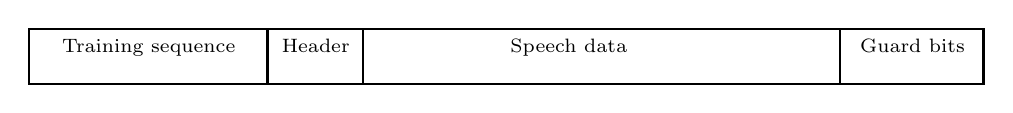
\begin{tikzpicture}[                
                    slot/.style={
            		text centered,
			font=\scriptsize,
			align=center,
			anchor=center,
			minimum height=0.7cm
            	}]
\draw[thick] (0,0) rectangle (\linewidth, -0.7);
\draw[thick] (0.25\linewidth,0) -- ++(0, -0.7);
\draw[thick] (0.35\linewidth,0) -- ++(0, -0.7);
\draw[thick] (0.85\linewidth,0) -- ++(0, -0.7);

\draw
(0,0) node[slot, minimum width=0.25\linewidth, anchor=north west](barker){Training sequence \\ \barkerBitsQPSK}
(0.25\linewidth,0)  node[slot, minimum width=0.1\linewidth, anchor=north west](barker){Header \\ \headerBits}
(0.35\linewidth,0) node[slot, minimum width=0.43\linewidth, anchor=north west](barker){Speech data \\ \packetDataBitsQPSK}
(0.85\linewidth,0) node[slot, minimum width=0.15\linewidth, anchor=north west](barker){Guard bits \\ \guardBitsQPSK}
;	

\end{tikzpicture}
}
  \\
  \subfloat[QAM-64 data package\label{1b}]{%
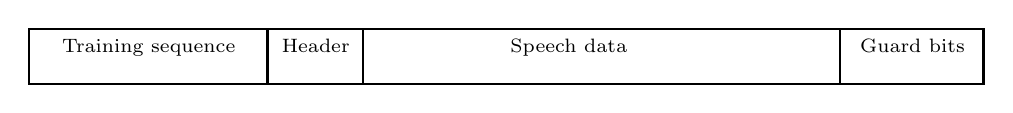
\begin{tikzpicture}[                
                    slot/.style={
            		text centered,
			font=\scriptsize,
			align=center,
			anchor=center,
			minimum height=0.7cm
            	}]
\draw[thick] (0,0) rectangle (\linewidth, -0.7);
\draw[thick] (0.25\linewidth,0) -- ++(0, -0.7);
\draw[thick] (0.35\linewidth,0) -- ++(0, -0.7);
\draw[thick] (0.85\linewidth,0) -- ++(0, -0.7);

\draw
(0,0) node[slot, minimum width=0.25\linewidth, anchor=north west](barker){Training sequence \\ \barkerBitsQAM}
(0.25\linewidth,0)  node[slot, minimum width=0.1\linewidth, anchor=north west](barker){Header \\ \headerBits}
(0.35\linewidth,0) node[slot, minimum width=0.43\linewidth, anchor=north west](barker){Speech data \\ \packetDataBitsQAM}
(0.85\linewidth,0) node[slot, minimum width=0.15\linewidth, anchor=north west](barker){Guard bits \\ \guardBitsQAM}
;	

\end{tikzpicture}}
\\
  \subfloat[QPSK BER package\label{1c}]{%
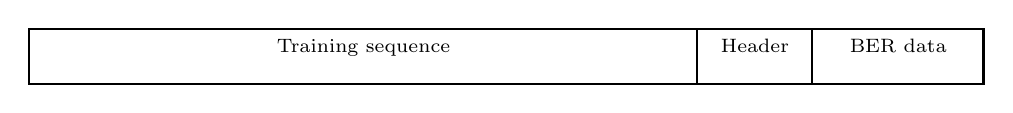
\begin{tikzpicture}[                
                    slot/.style={
            		text centered,
			font=\scriptsize,
			align=center,
			anchor=center,
			minimum height=0.7cm
            	}]
\draw[thick] (0,0) rectangle (\linewidth, -0.7);
\draw[thick] (0.70\linewidth,0) -- ++(0, -0.7);
\draw[thick] (0.82\linewidth,0) -- ++(0, -0.7);

\draw
(0,0) node[slot, minimum width=0.7\linewidth, anchor=north west](barker){Training sequence \\ \barkerBitsQPSK}
(0.70\linewidth,0)  node[slot, minimum width=0.12\linewidth, anchor=north west](barker){Header \\ \headerBits}
(0.82\linewidth,0) node[slot, minimum width=0.18\linewidth, anchor=north west](barker){BER data \\ \BERDataBits}
;	

\end{tikzpicture}}
  \caption{Burst format for QPSK(a) and QAM-64(b) modulated data bursts, and QPSK modulated BER burst (c)}
  \label{fig:burst_format} 
\end{figure}
